\chapter{Распространение ключей}\index{протокол!распространения ключей}\label{chapter-key-distribution-protocols}
\selectlanguage{russian}

Задача распространения ключей является одной из множества задач построения надёжной сети общения многих абонентов. Задача состоит в получении в нужный момент времени двумя легальными абонентами сети секретного сессионного ключа шифрования (и аутентификации сообщений). Хорошим решением данной задачи будем считать такой протокол распространения ключей, который удовлетворяет следующим условиям.

\begin{itemize}
	\item В результате работы протокола между двумя абонентами должен быть сформирован секретный сессионный ключ.
	\item Успешное окончание работы протокола распространения ключей должно означать успешную взаимную аутентификацию абонентов. Не должно быть такого, что протокол успешно завершился с точки зрения одной из сторон, а вторая сторона при этом представлена злоумышленником.
	\item К участию в работе протокола должны допускаться только легальные пользователи сети. Внешний пользователь не должен иметь возможность получить общий сессионный ключ с кем-либо из абонентов.
	\item Добавление нового абонента в сеть (или исключение из неё) не должно требовать уведомления всех участников сети.
\end{itemize}

Последнее требование сразу исключает такие варианты протоколов, в которых каждый из абонентов знал бы некоторый мастер-ключ общения с любым другим участником. Данные варианты плохи тем, что с ростом системы количество пар мастер-ключей <<абонент-абонент>> растёт как квадрат от количества участников. Поэтому большая часть рассматриваемых решений состоит в том, что в сети выделяется один или несколько доверенных центров T (\langen{Trent}, от \langen{trust}), которые как раз и владеют информацией обо всех легальных участниках сети и их ключах. Они же будут явно или неявно выступать одним из участников протоколов по формированию сеансовых ключей.

\begin{figure}[!htb]
    \centering
    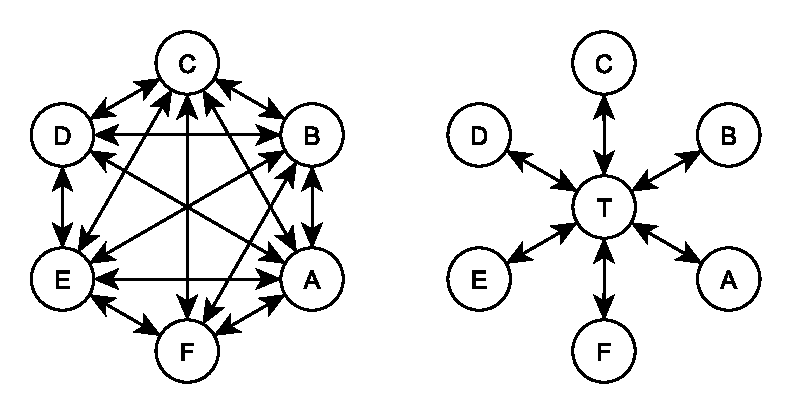
\includegraphics[width=0.8\textwidth]{pic/key_distribution-networks}
    \caption{Варианты сетей без выделенного доверенного центра и с выделенным доверенным центром T\label{fig:key_distribution-networks}}
\end{figure}

Важным моментом при анализе решений данной задачи является то, что сессионные ключи, вырабатываемые в конкретный момент времени, являются менее надёжными, чем мастер-ключи, используемые для генерации сессионных. В частности, нужно предполагать, что хотя злоумышленник не может получить сессионный ключ во время общения абонентов, он может сделать это по прошествии некоторого времени (дни, недели, месяцы). И хотя знание этого сессионного ключа поможет злоумышленнику расшифровать старые сообщения, он не должен иметь возможность организовать новую сессию с использованием уже известного ему сессионного ключа.

\input{key_distribution-simmetric}

\section{Трёхпроходные протоколы}
\selectlanguage{russian}

Если между Алисой и Бобом существует канал связи, недоступный для модификации злоумышленником (то есть когда применима модель только пассивного криптоаналитика), то даже без предварительного обмена секретными ключами или другой информацией можно воспользоваться идеями, использованными ранее в криптографии на открытых ключах. После описания RSA в 1978 году, в 1980 Ади Шамир предложил использовать криптосистемы, основанные на коммутативных операциях, для передачи информации без предварительного обмена секретными ключами. Если предположить, что передаваемой информацией является выработанной одной из сторон секретный сеансовый ключ, то в общем виде мы получаем следующий трёхпроходной протокол.

Предварительно:

\begin{itemize}
	\item Алиса и Боб соединены незащищённым каналом связи, открытым для прослушивания (но не для модификации) злоумышленником.
	\item Каждая из сторон имеет пару из открытого и закрытого ключей $K_A$, $k_A$, $K_B$, $k_B$ соответственно.
	\item Сторонами выбрана и используется коммутативная функция шифрования:
	\begin{align*}
		D_{A} \left( E_{A} \left( X \right) \right)	&= X		& ~~\forall ~ X, \left\{ K_A, k_a \right\}; \\
		E_{A} \left( E_{B} \left( X \right) \right)	&= E_B \left( E_A \left( X \right) \right) & ~~\forall ~ K_A, K_B, X.
	\end{align*}
\end{itemize}

Протокол состоит из трёх шагов (отсюда и название).
\begin{enumerate}
    \item Алиса создаёт новый секретный сеансовый ключ $K_S$, шифрует его с помощью своего ключа $K_A$ и посылает сообщение Бобу:
        \[ Alice \rightarrow ~ E_A \left( K_S \right) ~ \rightarrow Bob. \]
    \item Боб получает это сообщение, шифрует его с помощью своего ключа $K_B$ и посылает сообщение Алисе:
        \[ Bob \rightarrow ~ E_B \left( E_A \left( K_S \right) \right) ~ \rightarrow Alice. \]
    Алиса, получив сообщение $E_B \left( E_A \left( K_S \right) \right)$, использует свой закрытый ключ $k_A$ для расшифрования:
	\[ D_A \left( E_B \left( E_A \left( K_S \right) \right) \right) = D_A \left( E_A \left( E_B \left( K_S \right) \right) \right) = E_B \left( K_S \right). \]
    \item Алиса передаёт Бобу сообщение, в котором новый секретный сеансовый ключ зашифрован уже только ключом Боба:
        \[ Alice \rightarrow ~ E_B \left( K_S \right) ~ \rightarrow Bob. \]
    Боб, получив сообщение $E_B \left( K_S \right)$, использует свой ключ $k_B$ для расшифрования:
	\[ D_B \left( E_B \left( K_S \right) \right) = K_S. \]
\end{enumerate}

В результате стороны получают общий секретный ключ $K_S$.

Общим недостатком всех подобных протоколов является отсутствие аутентификации сторон. Конечно, в случае пассивного криптоаналитика это не требуется, но в реальной жизни всё-таки нужно рассматривать все возможные модели (в том числе активного криптоаналитика) и использовать такие протоколы, которые предполагают взаимную аутентификацию сторон.

\subsection{Тривиальный вариант}

Приведём пример протокола на основе функции XOR (побитовое сложение по модулю 2). Хотя данная функция может использоваться как фундамент для построения систем совершенной криптостойкости (см. главу~\ref{chapter:perfect_secure_systems}), для трёхпроходного протокола это неудачный выбор.

Перед началом протокола обе стороны имеют свои секретные ключи $K_A$ и $K_B$, представляющие собой случайные двоичные последовательности с равномерным распределением символов. Функция шифрования определяется как $E_i( X ) = X \oplus K_i$, где $X$ это сообщение, а $K_i$ -- секретный ключ. Очевидно, что:

\[ \forall i, j, X: E_i \left( E_j \left( X \right) \right) = X \oplus K_j \oplus K_i = X \oplus K_i \oplus K_j = E_j \left( E_i \left( X \right) \right) \]

\begin{enumerate}
    \item Алиса генерирует новый сеансовый ключ, шифрует его своим секретным ключом $K_A$ и посылает Бобу:
            \[\begin{array}{l}
		E_A(K) = K \oplus K_A, \\
		Alice \rightarrow ~ E_A(K) ~ \rightarrow Bob.
	    \end{array}\]
    \item Боб шифрует полученное сообщение уже своим ключом и отправляет Алисе:
            \[\begin{array}{l}
		E_B(E_A(K)) = K \oplus K_A \oplus K_B, \\
		Bob \rightarrow ~ E_B(E_A(K)) ~ \rightarrow Alice.
	    \end{array}\]
    \item Используя коммутативность операции шифрования, Алиса <<снимает>> шифрование своим ключом и отправляет результат Бобу:
            \[ D_A \left( E_B \left( E_A \left( K \right) \right) \right) = K \oplus K_A \oplus K_B \oplus K_A = K \oplus K_B = E_B \left( K \right). \]
            \[ Alice \rightarrow ~ E_B \left( K \right) ~ \rightarrow Bob. \]
    Боб, получив сообщение $K \oplus K_B$, выполняет расшифрование:
            \[ D_B( E_B( K ) ) = K \oplus K_B \oplus K_B = K. \]
    В результате Алиса и Боб знают общий сеансовый ключ $K$.
\end{enumerate}

Предложенный выбор коммутативной функции шифрования совершенной секретности был назван неудачным, так как существуют ситуации, при которых криптоаналитик может определить ключ $K$. Предположим, что криптоаналитик перехватил все три сообщения:
    \[ K \oplus K_A, ~~ K \oplus K_A \oplus K_B, ~~ K \oplus K_B. \]
Сложение по модулю 2 всех трёх сообщений даёт ключ $K$. Поэтому такая система шифрования не применяется.

Теперь приведём протокол надёжной передачи секретного ключа, основанный на экспоненциальной (коммутативной) функции шифрования. Стойкость этого протокола связана с трудностью задачи вычисления дискретного логарифма: известны значения $y, g, p$, найти $x$ в уравнении $y = g^x \mod p$.

\subsection{Бесключевой протокол Шамира}\index{протокол!Шамира бесключевой|(}

Стороны предварительно договариваются о большом простом числе $p \sim 2^{1024}$. Каждая из сторон выбирает себе по секретному ключу $a$ и $b$. Эти ключи меньше и взаимно просты с $p-1$. Также стороны приготовили по специальному числу $a'$ и $b'$, которые позволяют им расшифровать сообщение, зашифрованное своим ключом:

\[\begin{array}{l}
a' = a{-1} \mod (p-1), \\
a \times a' = 1 \mod (p-1), \\
\forall X: (X^a)^{a'} = X. \\
\end{array}\]

Последнее выражение верно по следствию из малой теоремы Ферма\index{теорема!Ферма малая}. Операции шифрования и расшифрования определяются следующим образом (на примере Алисы):

\[\begin{array}{ll}
\forall X < p:	& E_A( X ) = X^{a} \mod p, \\
		& D_A( X ) = X^{a'} \mod p, \\
		& D_A( E_A( X ) ) = X^{aa'} = X \mod p. \\
\end{array}\]

\begin{enumerate}
    \item Алиса создаёт новый сеансовый ключ $K < p$, шифрует его своим секретным ключом $a$ и посылает сообщение Бобу:
            \[\begin{array}{l}
		E_A(K) = K ^ a \mod p, \\
		Alice \rightarrow ~ E_A(K) ~ \rightarrow Bob.
	    \end{array}\]
    \item Боб шифрует полученное сообщение уже своим ключом и отправляет Алисе:
            \[\begin{array}{l}
		E_B(E_A(K)) = K^{ab} \mod p, \\
		Bob \rightarrow ~ E_B(E_A(K)) ~ \rightarrow Alice.
	    \end{array}\]
    \item Используя коммутативность операции шифрования, Алиса <<снимает>> шифрование своим ключом и отправляет результат Бобу:
            \[ D_A \left( E_B \left( E_A \left( K \right) \right) \right) = \left( K^{ab} \right) ^{a'} = K^{aa'b} = K^{b} = E_B \left( K \right) \mod p. \]
            \[ Alice \rightarrow ~ E_B \left( K \right) ~ \rightarrow Bob. \]
    Боб, получив сообщение $K \oplus K_B$, выполняет расшифрование:
            \[ D_B( E_B( K ) ) = K \oplus K_B \oplus K_B = K. \]
    В результате Алиса и Боб знают общий сеансовый ключ $K$.
\end{enumerate}

Предположим, что криптоаналитик перехватил три сообщения:
\[ \begin{array}{l}
    y_1 = K^a \mod p, \\
    y_2 = K^{ab} \mod p, \\
    y_3 = K^b \mod p. \\
\end{array} \]

Чтобы найти ключ $K$, криптоаналитику надо решить систему из этих трёх уравнений, что имеет очень большую вычислительную сложность, неприемлемую с практической точки зрения, если все три числа $a, b, ab$ достаточно велики. Предположим, что $a$ (или $b$) мало. Тогда, вычисляя последовательные степени $y_3$ (или $y_1$), можно найти $a$ (или $b$), сравнивая результат с $y_2$. Зная $a$, легко найти $a^{-1}\mod(p-1)$ и $K=(y_1)^{a^{-1}}\mod p$.

\index{протокол!Шамира бесключевой|)}

\subsection{Криптосистема Мэсси~---~Омуры}\index{протокол!Мэсси~---~Омуры|(}\index{криптосистема!Мэсси~---~Омуры|(}

В 1982 году Джеймс Мэсси и Джим Омура заявили патент (\langen{James Massey, Jim K. Omura},~\cite{Massey:Omura:1986}), улучшающий (по их мнению) бесключевой протокол Шамира. В качестве операции шифрования вместо возведения в степень в мультипликативной группе $\Z_p^*$ они предложили использовать возведение в степень в поле Галуа $\GF{2^n}$. Секретный ключ каждой стороны (для Алисы -- $a$) должен удовлетворять условиям:

\[ \begin{array}{l}
 a \in \GF{2^n}, \\
 gfd \left( a, x^{ n-1 } + x^{ n-2 } + ... + x + 1 \right) = 1. \\
\end{array} \]

В остальном протокол выглядит аналогично.

\index{протокол!Мэсси~---~Омуры|)}\index{криптосистема!Мэсси~---~Омуры|)}

\section{Асимметричные протоколы}

Асимметричные протоколы, или же протоколы, основанные на криптосистемах с открытыми ключами, позволяют ослабить требования к предварительному этапу протоколов. Вместо общего секретного ключа, который должны иметь две стороны (либо обе стороны и доверенный центр), в рассматриваемых ниже протоколах стороны должны предварительно обменяться открытыми ключами (между собой либо между собой и доверенным центром). Такой предварительный обмен может проходить по открытому каналу связи, в предположении, что криптоаналитик не может повлиять на содержимое канала связи на данном этапе.

\subsection{Простой протокол}

Рассмотрим протокол распространения ключей с помощью асимметричных шифров. Введём обозначения: $K_B$ -- открытый ключ стороны $B$, а $K_A$ -- открытый ключ стороны $A$. Протокол включает три сеанса обмена информацией.
\begin{enumerate}
    \item В первом сеансе сторона $A$ посылает стороне $B$ сообщение:
            \[ A \rightarrow B: ~ E_{K_B}(K_1, A), \]
        где $K_1$ -- ключ, выработанный стороной $A$.
    \item Сторона $B$ получает $(K_1, A)$ и передаёт стороне $A$ наряду с другой информацией свой ключ $K_2$ в сообщении, зашифрованном с помощью открытого ключа $K_A$:
            \[ A \leftarrow B: ~ E_{K_A}(K_2, K_1, B). \]
    \item Сторона $A$ получает и расшифровывает сообщение $(K_2, K_1, B)$. Во время третьего сеанса сторона $A$, чтобы подтвердить, что она знает ключ $K_2$, посылает стороне $B$ сообщение:
            \[ A \rightarrow B: ~ E_{K_B}(K_2). \]
\end{enumerate}
Общий ключ формируется из двух ключей: $K_1$ и $K_2$.

\subsection{Протоколы с цифровыми подписями}

Существуют протоколы обмена, в которых перед началом обмена ключами генерируются подписи сторон $A$ и $B$, соответственно $S_A(m)$ и $S_B(m)$. В этих протоколах можно использовать различные одноразовые метки. Рассмотрим пример.
\begin{enumerate}
    \item Сторона $A$ выбирает ключ $K$ и вырабатывает сообщение:
            \[ \left( K, ~ t_A, ~ S_A(K, t_A, B) \right), \]
        где $t_A$ -- метка времени. Зашифрованное сообщение передаёт стороне $B$:
        \[ A \rightarrow B: ~ E_{K_B}(K, ~ t_A, ~ S_A(K, t_A, B)). \]
    \item Сторона $B$ получает это сообщение, расшифровывает $\left( K, ~ t_A, ~ S_A(K, t_A, B) \right)$ и вырабатывает свою метку времени $t_B$. Проверка считается успешной, если $|t_B - t_A | < \delta $. Сторона $B$ знает свои реквизиты и может осуществлять проверку подписи.
\end{enumerate}

Имеется второй вариант протокола, в котором шифрование и подпись выполняются раздельно.
\begin{enumerate}
    \item Сторона $A$ вырабатывает ключ $K$, использует одноразовую метку (или метку времени) $t_{A}$ и передаёт стороне $B$ два различных зашифрованных сообщения:
            \[ \begin{array}{ll}
                A \rightarrow B: & ~ E_{K_B}(K, t_A), \\
                A \rightarrow B: & ~ S_A(K, t_A, B). \\
            \end{array} \]
    \item Сторона $B$ получает это сообщение, расшифровывает $K, t_A$ и, добавив свои реквизиты, может проверить подпись $S_A(K, t_A, B)$.
\end{enumerate}

В третьем варианте протокола сначала производится шифрование, потом подпись.
\begin{enumerate}
    \item Сторона $A$ вырабатывает ключ $K$, использует одноразовую случайную метку или метку времени $t_A$ и передаёт стороне $B$ сообщение:
        \[ A \rightarrow B: ~ t_A, ~ E_{K_B}(K, A), ~ S_A(t_A, ~ K, ~ E_{K_B}(K, A)). \]
    \item Сторона $B$ получает это сообщение, расшифровывает $\left( K, ~ A \right)$ и проверяет подпись $S_A(t_A, ~ K, ~ E_{K_B}(K, A))$.
\end{enumerate}

\subsection{Протокол Диффи~---~Хеллмана}\index{протокол!Диффи~---~Хеллмана}\label{section-protocols-diffie-hellman}
\selectlanguage{russian}

Первый алгоритм с открытым ключом был предложен Диффи и Хеллманом в работе 1976 года <<Новые направления в криптографии>> (\langen{Bailey Whitfield Diffie, Martin Edward Hellman, ``New directions in cryptography''},~\cite{Diffie:Hellman:1976}). Данный протокол, который также можно назвать \emph{схемой Диффи~---~Хеллмана}, стал первым, позволивший уменьшить требования к каналу связи для установления защищённого соединения без предварительного обмена ключами.

Протокол позволяет двум сторонам создать общий сеансовый ключ используя такой канал связи, который может прослушивать злоумышленник, но в предположении, что последний не может менять содержимое сообщений.

Пусть $p$ -- большое простое число\index{число!простое}, $g$ -- примитивный элемент группы $\Z_p^*$, ~ $y = g^x \bmod p$, причём $p, y, g$ известны заранее. Функцию $y=g^{x} \bmod p$ считаем однонаправленной, то есть вычисление функции при известном значении аргумента является лёгкой задачей, а её обращение (нахождение аргумента) при известном значении функции -- трудной.\footnote{Обратную функцию $x = \log_g y \bmod p$ называют функцией дискретного логарифма. В настоящий момент не существует быстрых способов вычисления такой функции для больших простых $p$.}

Протокол обмена состоит из следующих действий.

\begin{figure}
    \centering
    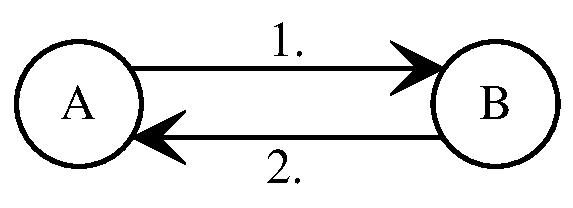
\includegraphics[width=0.5\textwidth]{pic/key_distribution-diffie-hellman}
    \caption{Общая схема взаимодействия участников в протоколе Диффи~---~Хеллмана\label{fig:key_distribution-diffie-hellman}}
\end{figure}

\begin{protocol}
    \item[(1)] Алиса выбирает случайное $2 \leq a \leq p - 1$
    \item[{}] $Alice \to \left\{ A = g ^ a \bmod p \right\} \to Bob$
    \item[(2)] Боб выбирает случайное $2 \leq b \leq p-1$
    \item[{}] Боб вычисляет сеансовый ключ $K = A ^ b \bmod p$
    \item[{}] $Bob \to \left\{ B = g ^ b \bmod p \right\} \to Alice$
    \item[(3)] Алиса вычисляет $K = B ^ a \bmod p$
\end{protocol}

Таким способом создан общий секретный сеансовый ключ $K$. За счёт случайного выбора значений $a$ и $b$ в новом сеансе будет получен новой сеансовый ключ.

Протокол обеспечивает только генерацию новых сеансовых ключей (цель G10). В отсутствие третей доверенной стороны он не обеспечивает ни аутентификацию сторон (цель G1), из-за отсутствия проходов с подтверждением владения ключом отсутствует аутентификация ключа (цель G8). Зато, так как протокол не использует длительные <<мастер>>-ключи, можно говорить о том, что он обладает свойством совершенной прямой секретности (цель G9).

Протокол можно использовать только с такими каналами связи, в которые не может вмешаться активный криптоаналитик. В противном случае протокол становится уязвим к простой <<атаке посередине>>.

\begin{figure}
    \centering
    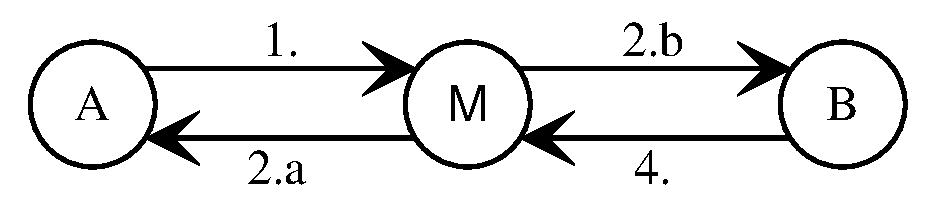
\includegraphics[width=0.67\textwidth]{pic/key_distribution-diffie-hellman-mitm}
    \caption{Схема взаимодействия участников в протоколе Диффи~---~Хеллмана в модели с активным криптоаналитиком\label{fig:key_distribution-diffie-hellman-mitm}}
\end{figure}

\begin{protocol}
    \item[(1)] Алиса выбирает случайное $2 \leq a \leq p - 1$
    \item[{}] $Alice \to \left\{ A = g ^ a \bmod p \right\} \to Mellory~(Bob)$
    \item[(2)] Меллори выбирает случайное $2 \leq m \leq p-1$
    \item[{}] Меллори вычисляет сеансовый ключ для канала с Алисой
        \[K_{AM} = A ^ m \bmod p = g ^ {am} \bmod p\]
    \item[{}] $Mellory~(Alice) \to \left\{ M = g ^ m \bmod p \right\} \to Bob$
    \item[{}] $Mellory~(Bob) \to \left\{ M = g ^ m \bmod p \right\} \to Alice$
    \item[(3)] Алиса вычисляет сеансовый ключ для канала с Меллори (думая, что Меллори это Боб)
        \[K_{AM} = M ^ a \bmod p = g ^ { am } \bmod p\]
    \item[(4)] Боб выбирает случайное $2 \leq b \leq p-1$
    \item[{}] Боб вычисляет сеансовый ключ для канала с Меллори (думая, что Меллори это Алиса)
        \[K_{BM} = M ^ b \bmod p = g ^ { bm } \bmod p\]
    \item[{}] $Bob \to \left\{ B = g ^ b \bmod p \right\} \to Mellory~(Alice)$
    \item[(5)] Меллори вычисляет сеансовый ключ для канала с Бобом
        \[K_{BM} = B ^ m \bmod p = g ^ { bm } \bmod p\]
\end{protocol}

В результате Алиса и Боб получили новые сеансовые ключи, но <<защищённый>> канал связи установили не с друг с другом, а со злоумышленником, который теперь имеет возможность ретранслировать или изменять все передаваемые сообщения между Алисой и Бобом.

Протокол Диффи~---~Хеллмана отличается от большей части протоколов распространения ключей из-за того, что не использует другие криптографические примитивы (функции шифрования, электронно-цифровой подписи или хеширования), но сам по себе является в некотором смысле криптографическим примитивом для построения более сложных протоколов. Он обеспечивает генерацию случайного числа в распределённой системе без доверенного центра. Причём ни одна из сторон не может заставить другую сторону использовать старый сессионный ключ, в отличие от, например, протокола Yahalom\index{протокол!Yahalom} из раздела~\ref{section-protocols-yahalom}.

Протокол можно изменить таким образом, чтобы вместо мультипликативной группы простого умножения использовать аддитивную группу сложения точек эллиптической кривой (см. раздел~\ref{section-math-ec-groups}). В этом случае стороны по прежнему будут выбирать некоторые случайные целые числа, но не возводить генератор-число в степень, а умножать генератор-точку на загаданное число.

\begin{protocol}
    \item[(0)] Стороны договорились о группе точек эллиптической кривой $\group{E}$, её циклической подгруппе $\group{G}$ мощности $n = \| \group{G} \|$ и генераторе $G$ группы $\group{G}$ (или хотя бы достаточно большой подгруппы группы $\group{G}$).
    \item[(1)] Алиса выбирает случайное $2 \leq a \leq n - 1$
    \item[{}] $Alice \to \left\{ A = a \times G \right\} \to Bob$
    \item[(2)] Боб выбирает случайное $2 \leq b \leq n - 1$
    \item[{}] Боб вычисляет точку $K = b \times A$
    \item[{}] $Bob \to \left\{ B = g \times G \right\} \to Alice$
    \item[(3)] Алиса вычисляет точку $K = a \times B$
\end{protocol}

В качестве нового сессионного ключа стороны могут выбрать, например, первую координату найденной точки $K$.


%\section{Протоколы с аутентификацией}

\subsection{Односторонняя аутентификация}

\textbf{Протокол Эль-Гамаля}\index{протокол!Эль-Гамаля} относится к протоколам с аутентификацией одного из двух легальных пользователей.
\selectlanguage{russian}
\begin{enumerate}
    \item Для начала стороны выбирают общие параметры $p, g$, где $p$ -- большое простое число, где $g$ -- примитивный элемент поля $\Z_p^*$.
    \item Сторона $B$ создает свои секретный и открытый ключи:
            \[ \SK_B = b, ~ \PK_B = g^b \mod p, \]
        $b$ -- случайное секретное число, $2 \leq b \leq p-1$.

        Открытый ключ $\PK_B$ находится в общем открытом доступе для всех сторон, поэтому криптоаналитик $E$ не может подменить его -- подмена будет заметна.
    \item Сторона $A$ вырабатывает свой секрет $x$, сеансовый ключ
            \[ K_A = (\PK_B)^x = g^{bx} \mod p \]
        и отправляет $B$:
            \[ A \rightarrow B: ~ g^x \mod p. \]
    \item Сторона $B$, получив от $A$ число $g^x \mod p$, использует его и свой секрет $\SK_B = b$, чтобы создать свой ключ
            \[ K_B = (g^x)^{\SK_B} = g^{bx} \mod p, \]
        то есть сеансовые ключи обеих сторон совпадают:
            \[ K_A = K_B = K. \]
\end{enumerate}

Достоинством этого протокола является следующее его свойство: если ключи $K_A$ и $K_B$ совпали и стороны могут обмениваться информацией, то сторона $A$ аутентифицирует сторону $B$, так как для шифрования она использовала открытый ключ $B$, который не может быть незаметно подменен, и только сторона $B$ может расшифровывать сообщения.

Что касается криптоаналитика в качестве <<человека-посередине>>, то он может отправлять ложные сообщения, но не может узнать ключ $K$ и читать сообщения.

Есть протоколы, в которых стороны, осуществляющие обмен информацией, являются равноправными. Они называются протоколами взаимной аутентификации.


\subsection{Взаимная аутентификация шифрованием}
\selectlanguage{russian}

К протоколам взаимной аутентификации принадлежит семейство протоколов, разработанных Т. Мацумото (T. Matsumoto), И. Такашима (Y. Takashima) и Х. Имаи (H. Imai) и названных по первым буквам фамилий авторов -- \textbf{протокол MTI}\index{протокол!MTI}.

Здесь к открытым данным относятся
    \[ p, ~~ g, ~~ \PK_A = g^a \mod p, ~~ \PK_B = g^b \mod p. \]
Каждый пользователь $A$ и $B$ обладает парой долговременных ключей для \emph{схемы шифрования с открытым ключом}: закрытый ключ расшифрования $\SK$ и открытый ключ шифрования  $\PK$.
\[ \begin{array}{ll}
    A: & ~ \SK_A = a, ~~ \PK_A = g^a \mod p, \\
    B: & ~ \SK_B = b, ~~ \PK_B = g^b \mod p. \\
\end{array} \]

\textbf{Протокол MTI}:
\begin{enumerate}
    \item Сторона $A$ генерирует случайное число $x, ~ 2\leq x\leq p-1$, создает и отправляет $B$ сообщение:
        \[ A \rightarrow B: ~ g^x \mod p. \]
    \item Сторона $B$ генерирует случайное число $y, ~ 2\leq y\leq p-1$, создает и отправляет $A$ сообщение:
        \[ A \leftarrow B: ~ g^y \mod p. \]
    \item Сторона $A$, используя открытые данные и полученное сообщение, создает сеансовый ключ:
        \[ K_A = (g^b)^x \cdot (g^y)^a = g^{bx+ay} \mod p. \]
    \item Сторона $B$, используя открытые данные и полученное сообщение, создает сеансовый ключ:
        \[ K_B = (g^x)^b \cdot (g^a)^y = g^{bx+ay} \mod p. \]
        Сеансовые ключи обоих сторон совпадают:
        \[ K_{A} =K_{B} = K. \]
\end{enumerate}

В описанном протоколе происходит взаимная аутентификация сторон как и в протоколе Эль-Гамаля\index{криптосистема!Эль-Гамаля}: открытые ключи сторон незаметно подменить невозможно. Наблюдая сообщения протокола, вычислить $g^{bx+ay}$ можно, только если известны значения $a,x$ или $b,y$, что представляет собой задачу дискретного логарифма, трудную в вычислительном смысле в настоящее время.


\subsection{Протокол Station-to-Station}\label{section-protocols-sts}\index{протокол!Station-to-Station|(}
\selectlanguage{russian}

Протокол STS (\langen{Station-to-Station},~\cite{Diffie:Oorschot:Wiener:1992})\index{протокол!Station-to-Station} предназначен для систем мобильной связи. Он использует идеи протокола Диффи~---~Хеллмана\index{протокол!Диффи~---~Хеллмана} и криптосистемы RSA\index{криптосистема!RSA}. Особенностью протокола является использование механизма электронной подписи\index{электронная подпись} для взаимной аутентификации сторон\index{аутентификация!взаимная}.

Предварительно стороны договорились об общих параметрах системы $p$ и $g$, где $p$ -- большое простое число, а $g$ -- примитивный элемент поля $\Z_p^*$.

Каждая из сторон $A$ и $B$ обладает долговременной парой ключей: закрытым ключом для расшифрования и создания электронной подписи $K_{\text{private}}$ и открытым ключом для шифрования и проверки подписи $K_{\text{public}}$.

\[\begin{array}{ll}
    A: K_{A,\text{private}}, K_{A,\text{public}}: \forall M : & \text{Verify}_A ( M, S_A( M ) ) = true, \\
                                                & D_A ( E_A( M ) ) = M, \\
    B: K_{B,\text{private}}, K_{B,\text{public}}: \forall M : & \text{Verify}_B ( M, S_B( M ) ) = true, \\
                                                & D_B ( E_B( M ) ) = M. \\
\end{array}\]

Где $\text{Verify}_A(\dots)$ это функция проверки электронной подписи на открытом ключе $K_{A, \text{public}}$, а $D_A$ -- функция расшифрования с использованием закрытого ключа $K_{A, \text{private}}$.

Протокол состоит из четырёх проходов, три из которых включают передачу сообщений (рис.~\ref{fig:key_distribution-sts}, \cite{Cheremushkin:2009}).

\begin{figure}
    \centering
    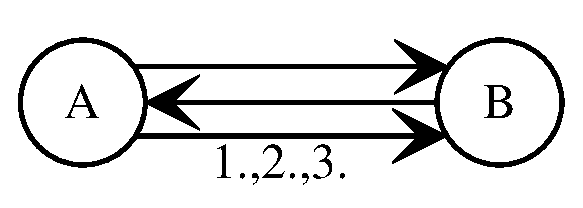
\includegraphics[width=0.5\textwidth]{pic/key_distribution-sts}
    \caption{Взаимодействие участников в протоколе STS\label{fig:key_distribution-sts}}
\end{figure}

\begin{protocol}
    \item[(1)] Алиса выбирает случайное число $R_A: 2 \leq R_A \leq p-1$.
    \item[{}] $Alice \to \left\{ A, m_A = g^{R_A} \bmod p \right\} \to Bob$

    \item[(2)] Боб выбирает случайное число $R_B: 2 \leq R_B \leq p-1$.
    \item[{}] Боб вычисляет сессионный ключ $K = m_A^{R_B} \bmod p$.
    \item[{}] $Bob \to \left\{ B, A, m_B = g^{R_B} \bmod p, E_K( S_B ( m_A, m_B )) \right\} \to Alice$

    \item[(3)] Алиса вычисляет сессионный ключ $K = m_B^{R_A} \bmod p$.
    \item[{}] Алиса проверяет подпись в сообщении $E_K( S_B ( m_A, m_B ))$.
    \item[{}] $Alice \to \left\{ A, B, E_K( S_A ( m_A, m_B ) ) \right\} \to Bob$

    \item[(4)] Боб проверяет подпись в сообщении $E_K( S_A ( m_A, m_B ))$.
\end{protocol}

Протокол обеспечивает гарантию формирования новых ключей (G10), но не совершенную прямую секретность (G9).

Как показала атака Лоу 1996 года (\cite{Lowe:1996}, рис.~\ref{fig:key_distribution-sts-attack}), протокол не может гарантировать аутентификацию субъектов (цель G1), ключей (G7) и подтверждение владения сессионным ключом (G8). Хотя злоумышленник не может получить доступ к новому сессионному ключу, если протокол использовать только для аутентификации субъектов, Алиса может принять злоумышленника за Боба.

\begin{figure}
    \centering
    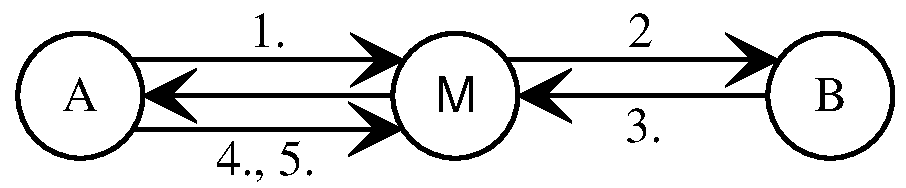
\includegraphics[width=0.67\textwidth]{pic/key_distribution-sts-attack}
    \caption{Схема взаимодействия участников в протоколе STS при атаке Лоу\label{fig:key_distribution-sts-attack}}
\end{figure}

\begin{protocol}
    \item[(1)] Алиса выбирает случайное число $R_A: 2 \leq R_A \leq p-1$.
    \item[{}] $Alice \to \left\{ A, m_A = g^{R_A} \bmod p \right\} \to Mellory~(Bob)$

    \item[(2)] $Mellory~(Alice) \to \left\{ M, m_A \right\} \to Bob$

    \item[(3)] Боб выбирает случайное число $R_B: 2 \leq R_B \leq p-1$ и вычисляет $m_B = g^{R_B} \bmod p$, а также сессионный ключ $K = m_A^{R_B} \bmod p$.
    \item[{}] $Bob \to \left\{ B, M, m_B, E_K( S_B ( m_A, m_B )) \right\} \to Mellory$

    \item[(4)] $Mellory~(Bob) \to \left\{ B, A, m_B, E_K( S_B ( m_A, m_B )) \right\} \to Alice$

    \item[(5)] Алиса вычисляет сессионный ключ $K = m_B^{R_A} \bmod p$.
    \item[{}] Алиса проверяет подпись в сообщении $E_K( S_B ( m_A, m_B ))$.
    \item[{}] $Alice \to \left\{ A, B, E_K( S_A ( m_A, m_B ) ) \right\} \to Mellory~(Bob)$
\end{protocol}

После успешного завершения протокола Алиса уверена, что общается с Бобом.

Как и все остальные <<криптосистемы-протоколы>>, протокол Station-to-Station основывается на некотором внешнем источнике информации об открытых ключах участников, не подвергая сомнению корректность и надёжность этого источника. Что, в общем случае, неверно. Если информацию о ключах участников нужно получать извне при каждом сеансе протокола (например, если участников много, и запомнить ключи всех возможности нет), то канал получения открытых ключей будет основной целью активного криптоаналитика для рассмотренных протоколов. Как от этого защититься с использованием примитивов асимметричной криптографии -- в разделе~\ref{section-protocols-asymmetric}.

\index{протокол!Station-to-Station|)}

\subsection{Схема Жиро}\label{section-girault-scheme}\index{схема!Жиро|(}
\selectlanguage{russian}

В схеме Жиро (\langfr{Marc Girault},~\cite{Girault:1990, Girault:1991}) надёжность строится на стойкости криптосистемы RSA (сложности факторизации больших чисел и вычисления дискретного корня).

Предварительно:
\begin{itemize}
    \item Доверенный центр (Трент, $T$):
    \begin{itemize}
        \item выбирает общий модуль $n = p \times q$, где $p$ и $q$ -- большие простые числа;
        \item выбирает пару из закрытого и открытого ключей $K_{T, \text{public}}: (e, n)$ и $K_{T, \text{private}}: (d, n)$;
        \item выбирает элемент $g$ поля $\mathbb{Z}_n^{\times}$ максимального порядка;
        \item публикует в общедоступном месте параметры схемы $n$, $e$ и $g$.
    \end{itemize}
    \item Каждый из легальных участников:
    \begin{itemize}
        \item выбирает себе закрытый ключ $s_i$ и идентификатор $I_i$;
        \item вычисляет и отправляет доверенному центру $v_i = g^{-s_i} \bmod n$;
        \item используя протокол аутентификации сторон (см. ниже) легальный участник доказывает доверенному центру, что владеет закрытым ключом, не раскрывая его значение;
        \item получает от доверенного центр свой открытый ключ:
            \[ P_i = (v_i - I_i)^d = (g^{-s_i} - I_i)^d \mod n; \]
    \end{itemize}
    В результате для каждого участника, например, Алисы, которая владеет $P_A, I_A, s_a$ будет выполняться утверждение:
        \[ P_A^e + I_A = g^{-s_A} \mod n. \]
\end{itemize}

Протокол аутентификации сторон в общем случае выглядит следующим образом (рис.~\ref{fig:key_distribution-girault-auth}).

\begin{figure}
    \centering
    \includegraphics[width=0.5\textwidth]{pic/key_distribution-girault-auth}
    \caption{Взаимодействия участников в протоколе идентификации Жиро\label{fig:key_distribution-girault-auth}}
\end{figure}

\begin{protocol}
    \item[(1)] Алиса выбирает случайное $R_A$.
    \item[{}] $Alice \to \left\{ I_A, P_A, t = g^{R_A} \right\} \to Bob$
    \item[(2)] Боб выбирает случайное $R_B$.
    \item[{}] $Bob \to \left\{ R_B \right\} \to Alice$
    \item[(3)] $Alice \to \left\{ y = R_A + s_A \times R_B \right\} \to Bob$
    \item[(4)] Боб вычисляет $v_A = P_A^e + I_A$;
    \item[{}] Боб проверяет, что $g^ y v_A^{R_B} = t$.
\end{protocol}

Протокол генерации сессионного ключа, либо просто \emph{схема Жиро}, как и другие схемы, состоит из проходов обмена открытой информацией и вычисления ключа (рис.~\ref{fig:key_distribution-girault-scheme}).

\begin{figure}
    \centering
    \includegraphics[width=0.5\textwidth]{pic/key_distribution-girault-scheme}
    \caption{Взаимодействие участников в схеме Жиро\label{fig:key_distribution-girault-scheme}}
\end{figure}

\begin{protocol}
    \item[(1)] $Alice \to \left\{ P_A, I_A \right\} \to Bob$
    \item[(2)] Боб вычисляет $K_{BA} = (P_A^e + I_A)^{s_B} \bmod n$.
    \item[{}] $Bob \to \left\{ P_B, I_B \right\} \to Alice$
    \item[(3)] Алиса вычисляет $K_{AB} = (P_B^e + I_B)^{s_A} \bmod n$.
\end{protocol}

В результате работы схемы стороны сгенерировали одинаковый общий сеансовый ключ.
\[ K_{AB} = (P_A^e + I_A)^{s_B} = (g^{-s_A})^{s_B} = g^{-s_As_B} \mod n; \]
\[ K_{BA} = (P_B^e + I_B)^{s_A} = (g^{-s_B})^{s_A} = g^{-s_As_B} \mod n; \]
            \[ K = K_{AB} = K_{BA} = g^{-s_As_B} \mod n. \]

Схема обеспечивает аутентификацию ключа (цель G7), так как только легальные пользователи смогут вычислить корректное значение общего сессионного ключа.

\index{схема!Жиро|)}

\subsection{Схема Блома}\index{схема!Блома}
\selectlanguage{russian}

Рассмотрим распределение ключей по \emph{схеме Блома} (Rolf Blom,~\cite{Blom:1984, Blom:1985}), в котором каждые два пользователя из общего числа $N$ пользователей могут создать общий секретный ключ, причём секретные ключи каждой пары различны. Данная схема используется в протоколе HDCP\index{протокол!HDCP} (\langen{High-bandwidth Digital Content Protection}) для предотвращения копирования высококачественного видеосигнала.

На этапе инициализации доверенный центр выбирает симметричную матрицу $D_{m,m}$ над конечным полем $\GF p$. Для присоединения к сети распространения ключей новый участник либо самостоятельно, либо с помощью доверенного центра выбирает новый открытый ключ (идентификатор) $I$, представляющий собой вектор длины $k$ над $\GF p$. Доверенный центр вычисляет для нового участника закрытый ключ $K$:

\begin{equation}
	K = D_{m,m} I.
	\label{eq:blom_center_matrix}
\end{equation}

Симметричность матрицы $D_{m,m}$ доверенного центра позволяет любым двум участникам сети создать общий сеансовый ключ. Пусть Алиса и Боб -- легальные пользователи сети, то есть они обладают открытыми ключами $I_A$ и $I_B$ соответственно, а их закрытые ключи $K_A$ и $K_B$ были вычислены одним и тем же доверенным центром по формуле~\ref{eq:blom_center_matrix}. Тогда протокол выработки общего секретного ключа выглядит следующим образом.

\begin{enumerate}
	\item Алиса отправляет Бобу свой открытый ключ $I_A$.
	\item Боб отправляет Алисе свой открытый ключ $I_B$.
	\item Алиса вычисляет значение $s_{AB} = K^t_A I_B = I^t_A D_{m,m} I_B$.
	\item Боб вычисляет значение $s_{BA} = K^t_B I_A = I^t_B D_{m,m} I_A$.
\end{enumerate}

Из симметричности матрицы $D_{m,m}$ следует, что значения $s_{AB}$ и $s_{BA}$ совпадут, они же и будут являться общим секретным ключом для Алисы и Боба. Этот секретный ключ будет свой для каждой пары легальных пользователей сети.

Присоединение новых участников к схеме строго контролируется доверенным центром, что позволяет защитить сеть от нелегальных пользователей. Надёжность данной схемы основывается на невозможности восстановить исходную матрицу. Однако для восстановления матрицы доверенного центра размера $m \times m$ необходимо и достаточно всего $m$ пар линейно независимых открытых и закрытых ключей. В 2010 году компания Intel, которая является <<доверенным центром>> для пользователей системы защиты HDCP, подтвердила, что криптоаналитикам удалось найти секретную матрицу (точнее, аналогичную ей), используемую для генерации ключей в упомянутой системе предотвращения копирования высококачественного видеосигнала.


\section{Квантовые протоколы}\index{протокол!квантовые|(}

\subsection{Протокол BB84}\index{протокол!BB84|(}
\selectlanguage{russian}

В 1984 году Чарлз Беннет (\langen{Charles Henry Bennett}) и Жиль Брассар (\langfr{Gilles Brassard}) предложили новый квантовый протокол распределения ключа~\cite{Bennett:Brassard:1984}. Как и у других протоколов, его целью является создание нового сеансового ключа, который в дальнейшем можно использовать в классической симметричной криптографии. Однако особенностью протокола является использование отдельных положений квантовой физики для гарантии защиты получаемого ключа от перехвата злоумышленником.

До начала очередного раунда генерации сеансового ключа предполагается, что у Алисы и Боба, как у участников протокола, имеется:

\begin{itemize}
	\item квантовый канал связи (например, оптоволокно);
	\item классический канал связи;
\end{itemize}

Протокол гарантирует, что вмешательство злоумышленника в протокол можно заметить вплоть до тех пор, пока злоумышленник не сможет контролировать и на чтение, и на запись все каналы общения сразу.

Протокол состоит из следующих этапов:

\begin{itemize}
	\item передача и приём фотона по квантовому каналу связи от Алисы к Бобу;
	\item передача Бобом информации об использованных анализаторах;
	\item передача Алисой информации о совпадении выбранных анализаторов и исходных поляризаций.
\end{itemize}


\subsubsection{Генерация фотона}

В первой части протокола с точки зрения физика-экспериментатора Алиса берёт единичный фотон и поляризует под одним из четырёх углов: 0, 45, 90 или 135. Будем говорить, что Алиса сначала выбрала базис поляризации (<<+>> или <<?>>), а затем выбрала в этом базисе одно из двух направлений поляризации:

\begin{itemize}
	\item $0^{\circ}$ (<<$\rightarrow$>>) или $90^{\circ}$ (<<$\uparrow$) в первом базисе (<<+>>);
	\item $45^{\circ}$ (<<$\nearrow$>>) или $135^{\circ}$ (<<$\nwarrow$) во втором базисе (<<×>>).
\end{itemize}

С точки зрения квантовой физики мы можем считать, что у нас есть система с двумя базовыми состояниями $|0\rangle$ и $|1\rangle$. Состояние системы в любой момент времени можно записать как $| \psi \rangle = \cos \alpha |0\rangle + \sin \beta |1\rangle$. Так как четыре выбранных Алисой возможных исходных состояния неортогональны между собой (точнее, не все попарно), то из законов квантовой физики следует два важных момента:

\begin{itemize}
	\item невозможность клонировать состояние фотона;
	\item невозможность достоверно отличить неортогональные состояния друг от друга.
\end{itemize}

С точки зрения специалиста по теории информации можем считать, что Алиса использует две независимые случайные величины $X_A$ и $A$ с энтропией по 1 бит каждый, чтобы получить новую случайную величину $Y_A = f \left( X_A; A \right)$, передаваемую в канал связи.

\begin{itemize}
	\item $H \left( A \right) = 1~\text{бит}$, выбор базиса поляризации (<<+>> или <<×>>);
	\item $H \left( X \right) = 1~\text{бит}$, само сообщение, выбор одного из двух направлений поляризации в базисе.
\end{itemize}

\subsubsection{Действия злоумышленника}

Как физик-экспериментатор Ева может попытаться встать посередине канала и что-то с фотоном сделать. Может попытаться просто уничтожить фотон или послать вместо него случайный. Хотя последнее приведёт к тому, что Алиса и Боб не смогут сгенерировать общий сеансовый ключ, полезную информацию Ева из этого не извлечёт.

Ева может попытаться пропустить фотон через один из поляризаторов и попробовать поймать фотон детектором. Если бы Ева точно знала, что у фотона может быть только два ортогональных состояния (например, вертикальная <<$\uparrow$>> или горизонтальная <<$\rightarrow$>> поляризация), то она могла бы вставить на пути фотона вертикальный поляризатор <<$\uparrow$>> и по наличию сигнала на детекторе определить, была ли поляризация фотона вертикальной (1, есть сигнал) или горизонтальной (0, фотон через поляризатор не прошёл и сигнала нет). Проблема Евы в том, что у фотона не два состояния, а четыре. И никакое положение одного поляризатора и единственного детектора не поможет Еве точно определить, какое из этих четырёх состояний принимает фотон. А пропустить фотон через два детектора не получится. Во-первых, если фотон прошёл вертикальный  поляризатор, то какой бы исходной у него не была поляризация (<<$\nwarrow$>>, <<$\uparrow$>>, <<$\nearrow$>>), после поляризатора она станет вертикальной <<$\uparrow$>> (вторая составляющая <<сотрётся>>). Во-вторых, детектор, преобразуя фотон в электрический сигнал, тем самым уничтожает его, что несколько затрудняет его дальнейшие измерения.

Кроме того, двух или даже четырёх детекторов для одного фотона будет мало. Отличить между собой неортогональные поляризации <<$\uparrow$>> и <<$\nearrow$>> можно только статистически, так как каждая из них будет проходить и вертикальный <<$\uparrow$>>, и диагональный <<$\nearrow$>> поляризаторы, но с разными вероятностями (100\% и 50\%).

С точки зрения квантовой физики Ева может попытаться провести измерение фотона, что приводит к \emph{коллапсу волновой функции} (или же \emph{редукции фон Неймана}) фотона. То есть после действия оператора измерения на волновую функцию фотона она неизбежно меняется, что приведёт к помехам в канале связи, которые могут обнаружить Алиса и Боб. Невозможность достоверно отличить неортогональные состояния мешает Еве получить полную информацию о состоянии объекта, а запрет клонирования мешает повторить измерение с дубликатом системы.

С точки зрения теории информации мы можем рассмотреть фактически передаваемое состояние фотона как некоторую случайную величину $Y_A$. Ева использует случайную величину $E$ (выбор пары ортогональных направлений поляризатора – <<+>> либо <<×>>) для получения величины $Y_E$ как результата измерения $Y_A$. При этом для каждого заданного исходного состояния Ева получает на выходе:

\begin{itemize}
	\item аналогичное состояние с вероятностью 50\% (вероятность выбора пары ортогональных направлений поляризатора, совпадающих с выбранной Алисой);
	\item одно из двух неортогональных оригинальному состояний с вероятностью 25\% каждое.
\end{itemize}

Таким образом, условная энтропия величины $Y'$, измеренной Евой, относительно величины Y, переданной Алисой, равна:

\[ H \left( Y_E | Y_A \right) = - \frac{1}{2} \log_2 \frac{1}{2} - \frac{1}{4} \log_2 \frac{1}{4} - \frac{1}{4} \log_2 \frac{1}{4} = 1,5~\text{бит}. \]

И взаимная информация между этими величинами равна:
\[ I \left( Y_E ; Y_A \right) = H \left( Y_E \right) - H ( Y_E | Y_A ) = 0,5~\text{бит}.\]

Что составляет 25\% от энтропии, передаваемой по каналу случайной величины $Y$.

Если рассматривать величину $X_E$, которую Ева пытается восстановить из принятой ею величины $Y_E$, то с точки зрения теории информации ситуация ещё хуже:

\begin{itemize}
	\item при угаданном базисе поляризатора получаем исходную величину $X_E = X_A$;
	\item при неугаданном базисе ещё в половине случаев получаем исходную величину (из-за случайного прохождения фотона через <<неправильный>> поляризатор).
\end{itemize}

Получается, что условная энтропия восстанавливаемой Евой последовательности $X_E$ относительно исходной $X_A$ равна:
\[ H \left( X_E | X_A \right) = - \frac{3}{4} \log \frac{3}{4} – \frac{1}{4} \log \frac{1}{4} \approx 0,81~\text{бит.}\]

И взаимная информация
\[ I \left( X_E; X_A \right) = H \left( X_E \right) - H \left( X_E | X_A \right) \approx 0,19~~\text{бит}. \]

Что составляет $\approx 19\%$ от энтропии исходной случайной величины $X_A$.

Оптимальным алгоритмом дальнейших действий Евы будет послать Бобу фотон в полученной поляризации (передать далее в канал полученную случайную величину $Y_E$). То есть если Ева использовала вертикальный поляризатор <<$\uparrow$>>, и детектор зафиксировал наличие фотона, то передавать фотон в вертикальной поляризации <<$\uparrow$>>, а не пытаться вводить дополнительную случайность и передавать <<$\nwarrow$>> или <<$\nearrow$>>.

\subsubsection{Действия легального получателя}

Боб, аналогично действиям Евы (хотя это скорее Ева пытается имитировать Боба), случайным образом выбирает ортогональную пару направлений поляризации (<<+>> либо <<×>>) и ставит на пути фотона поляризатор (<<$\uparrow$>> или <<$\nwarrow$>>) и детектор. В случае наличия сигнала на детекторе он записывает единицу, в случае отсутствия – ноль.

Аналогично Еве, можно сказать, что Боб вводит новую случайную величину B (отражает выбор базиса поляризации Бобом) и в результате измерений получает новую случайную величину $X_B$. Причём Бобу пока неизвестно, использовал ли он оригинальный сигнал $Y_A$, переданный Алисой, или же подложный сигнал $Y_E$Y, переданный Евой:

\begin{itemize}
	\item $X_{B1} = f \left( Y_A, B \right);$
	\item $X_{B2} = f \left( Y_E, B \right).$
\end{itemize}

Далее Боб сообщает по открытому общедоступному классическому каналу связи, какие именно базисы поляризации использовались, а Алиса указывает, какие из них совпали с изначально выбранными. При этом сами измеренные значения (прошёл фотон через поляризатор или нет) Боб оставляет в секрете.

Можно сказать, что Алиса и Боб публикуют значения сгенерированных ими случайных величин $A$ и $B$. Примерно в половине случаев эти значения совпадут (когда Алиса подтверждает правильность выбора базиса поляризации). Для тех фотонов, у которых значения $A$ и $B$ совпали, совпадут и значения $X_A$ и $X_{B1}$. То есть:

\begin{itemize}
	\item $H \left( X_{B1} | X_A; A = B \right) = 0~\text{бит}$,
	\item $I \left( X_{B1} ; X_A | A = B \right) = 1~\text{бит}$.
\end{itemize}

Для тех фотонов, для которых Боб выбрал неправильный базис поляризации, значения $X_{B1}$ и $X_{A}$ будут представлять собой независимые случайные величины (так как, например, при исходной диагональной поляризации фотона он пройдёт и через вертикальную, и через горизонтальную щель с вероятностью 50\%):

\begin{itemize}
	\item $H \left( X_{B1} | X_A; A \neq B \right) = 1~\text{бит},$
	\item $I \left( X_{B1} ; X_A | A \neq B \right) = 0~\text{бит}.$
\end{itemize}

Рассмотрим случай, когда Ева вмешалась в процесс передачи информации между Алисой и Бобом и отправляет Бобу уже свои фотоны, но не имеет возможности изменять информацию, которой Алиса и Боб обмениваются по классическому каналу связи. Как и прежде, Боб отправляет Алисе выбранные базисы поляризации (значения $B$), а Алиса указывает, какие из них совпали с выбранными ею значениями $A$.

Но теперь, для того, чтобы Боб получил корректное значение $X_{B2}$ ($X_{B2} = X_A$), должны быть выполнены все следующие условия для каждого фотона:

\begin{itemize}
	\item Ева должна угадать базис поляризации Алисы ($E = A$).
	\item Боб должен угадать базис поляризации Евы ($B = E$).
\end{itemize}

Рассмотрим без ограничения общности вариант, когда Алиса использовала диагональную поляризацию <<×>>:

\begin{tabular}{ | c | c | c | c | }
\hline
Базис & Базис & Базис & \\
Алисы & Евы & Боба & Результат \\
\hline
<<×>> & <<×>> & <<×>> & принято без ошибок \\
<<×>> & <<×>> & <<+>> & отклонено \\
<<×>> & <<+>> & <<×>> & принято с ошибками\\
<<×>> & <<+>> & <<+>> & отклонено \\
\hline
\end{tabular}

При этом Боб и Алиса будут уверены, что в первом и третьем случае (которые с их точки зрения ничем не отличаются), Боб корректно восстановил поляризацию фотонов. Так как все эти строки равновероятны, то получается, что у Боба и Алисы после выбора только фотонов с <<угаданным>> базисами (как они уверены) только половина поляризаций (значений $X_A$ и $X_{B2}$) будет совпадать. При этом Ева будет эти значения знать. Количество известных Еве бит <<общей>> последовательности и доля ошибок в ней находятся в линейной зависимости от количества перехваченных Евой бит.

Вне зависимости от наличия или отсутствия Евы Алиса и Боб вынуждены использовать заранее согласованную процедуру исправления ошибок. Используемый код коррекции ошибок, с одной стороны, должен исправлять ошибки, вызванные физическими особенностями квантового канала. Но с другой стороны, если код будет исправлять слишком много ошибок, то он скроет от нас потенциальный факт наличия Евы. Доказано, что существуют такие методы исправления ошибок, которые позволяют безопасно (без опасности раскрыть информацию Еве) исправить от 7,5\% (Майерз, 2001, \cite{Mayers:2001}) до 11\% ошибок (Ватанабе, Матсумото, Уйематсу, 2005,~\cite{Watanabe:Matsumoto:Uyematsu:2005}).

Интересен также вариант, когда Ева может изменять информацию, передаваемую не только по оптическому, но и по классическому каналам связи. В этом случае многое зависит от того, в какую сторону (от чьего имени) Ева может подделывать сообщения. В самом негативном сценарии, когда Ева может выдать себя и за Алису, и за Боба, будет иметь место полноценная атака <<человек-посередине>> (\langen{man-in-the-middle}), от которой невозможно защититься никаким способом, если не использовать дополнительные защищённые каналы связи, или не основываться на информации, переданной заранее. Однако, это будет уже совсем другой протокол.

Подводя итоги, квантовые протоколы распределения ключей (а именно ими пока что и ограничивается вся известная на сегодняшний день <<квантовая криптография>>), обладают как определёнными особенностями, так и фатальными недостатками, затрудняющими их использование (и ставящими под вопрос саму эту необходимость):

\begin{itemize}
	\item Любые квантовые протоколы (как и вообще любые квантовые вычисления) требуют оригинального дорогостоящего оборудования, которое пока что нельзя сделать частью commodity-устройств или обычного сотового телефона.
	\item Квантовые каналы связи -- это всегда физические каналы связи. У них существует максимальная длина канала и определённый уровень ошибок. Для квантовых каналов (на сегодняшний день) не придумали <<повторителей>>, которые бы позволили бы увеличить длину безусловно квантовой передачи данных.
	\item Ни один квантовый протокол (на сегодняшний день) не может обходиться без дополнительного классического канала связи. Для такого связи требуются как минимум такой же уровень защиты, как и при использовании, например, криптографии с открытым ключом.
	\item Для всех протоколов особую проблему представляет не только доказательство корректности (что является весьма нетривиальным делом в случае наличия <<добросовестных>> помех), но и инженерная задача по реализации протокола в <<железе>>. В качестве краткой иллюстрации, например, не существует простого способа создать <b>ровно один</b> фотон. Недогенерация фотонов приводит, очевидно, к ошибкам передачи, а генерация дубля в том же временном слоте -- к возможностью его перехвата злоумышленником без создания помех в канале.
\end{itemize}

\index{протокол!BB84|)}
\index{протокол!квантовые|)}

